\section{Applications and Performance Evaluation}
\label{clicknp:sec:application}
\label{clicknp:sec:eval}

To assess the adaptability of \name, several standard network functions were developed based on \name, which can operate in the testbed of this study. Table \ref {clicknp:tab:applications} encapsulates the number of elements and total lines of code included in each network function, encompassing all element specifications and configuration files. It has been confirmed that the modular architecture of \name significantly enhances code reusability and simplifies the development of new network functions. As depicted in Table \ref {clicknp:tab:elements}, there are numerous opportunities to reuse an element in many applications, for instance, all network functions in this study utilize L4\_Parser. Each network function may take approximately 1 hour for a programmer to develop and debug. The capability to process in conjunction with CPU / FPGA will also significantly aid debugging, as problematic elements can be transferred to the CPU for easy log printing to trace issues.

This chapter evaluates \name in a testbed of 16 Dell R720 servers. For each FPGA board, two Ethernet ports are connected to the Top-of-Rack Dell S6000 switch\cite {dells6000}. All \name network functions operate on Windows Server 2012 R2. This chapter contrasts \name with other cutting-edge software network functions. For those network functions operating on Linux, CentOS 7.2 with kernel version 3.10 is utilized. The test employs the PktGen packet sending tool to generate test traffic at varying rates with different packet sizes (64B packets, maximum throughput is 56.4 Mpps). To measure the processing delay of network functions, a generation timestamp is embedded in each test packet. When the packets traverse the network function, they are looped back to the PktCap packet capture tool, which is located in the same FPGA as PktGen. Then the delay can be determined by subtracting the generation timestamp from the packet reception time. The delay caused by PktGen and PktCap is pre-calibrated by direct loopback (without network function) and removed from the data.

The following sections introduce the network functions based on \name in sequence.

\egg{
To measure the processing latency of network functions, we forward packets to an \textit{Echo} server using the second port. 
The Echo server operates an \textit{Echo} function in its FPGA, which simply reflects all packets back to the source. 
%
We can then compare the difference between the timestamps of a packet 
when it initially arrives and when the processed packet is reflected back, to determine the latency 
with nanosecond precision.
%
The delay caused by the Echo server was pre-calibrated and subtracted from our data.
In our test, we use PktGen to generate testing traffic, which can 
produce packets at a rate of up to 56.4 Mpps (64B packets).
}

\egg{
Ethernet ports of FPGAs and servers are connected to a Dell S6000 40GbE switch 
FPGAs are installed on Windows Server 2012 R2.
CPU-based benchmarks are performed on 

We use the TrafficGen application to benchmark throughput and latency.
The TrafficGen application generates a given traffic pattern or replays a trace, embeds a timestamp in the packet payload, and sends it to tor\_out.
Applications forward packets from tor\_in to nic\_out. When TrafficGen receives a packet from nic\_in, the timestamp is extracted from the payload to measure latency.
The wire loopback RTT of TrafficGen is 0.85$\mu$s for 64B packets and 1.39$\mu$s for 1504B packets, which is the system error in all latency numbers we present.
}

\subsection{Packet Generator and Packet Capture Tools}
The Packet Generator (PktGen) can generate various traffic patterns based on different configuration files. It can produce streams of different sizes and schedule them to start at different times according to a given distribution. The generated streams can be further controlled in terms of flow rate and burstiness through different traffic shapers.

The Packet Capture Tool (PktCap) redirects all received packets to \textit{logger} components, which are typically located in the host. Figure \ref{clicknp:fig:packet-capture} illustrates the component structure of the packet capture tool. Since a single packet capture component cannot fully utilize the capacity of the PCIe I/O channel, PktCap implements a Receive Side Scaling (RSS) component in the FPGA to distribute packets to multiple packet capture components based on the hash value of the flow 5-tuple. Due to the throughput of the PCIe channel being less than the throughput of the 40G network card, an \textit{extractor} component is added, which only extracts important fields of the packet (for example, if there are 5 tuples, DSCP and VLAN tags), and forwards these fields (a total of 16B) and the timestamp (4B) via PCIe. PktCap is an example of demonstrating the importance of joint CPU / FPGA processing. Compared with FPGA, the CPU has more memory for buffering and can easily access other storage, such as the HDD / SSD drives in the literature \cite{lee2015flosis}, so it is more logical to run the logger on the CPU.

The content you provided is already in English and in an academic style. As per your instructions, I will not make any changes to it.

\begin{figure}[htbp]
	\centering
	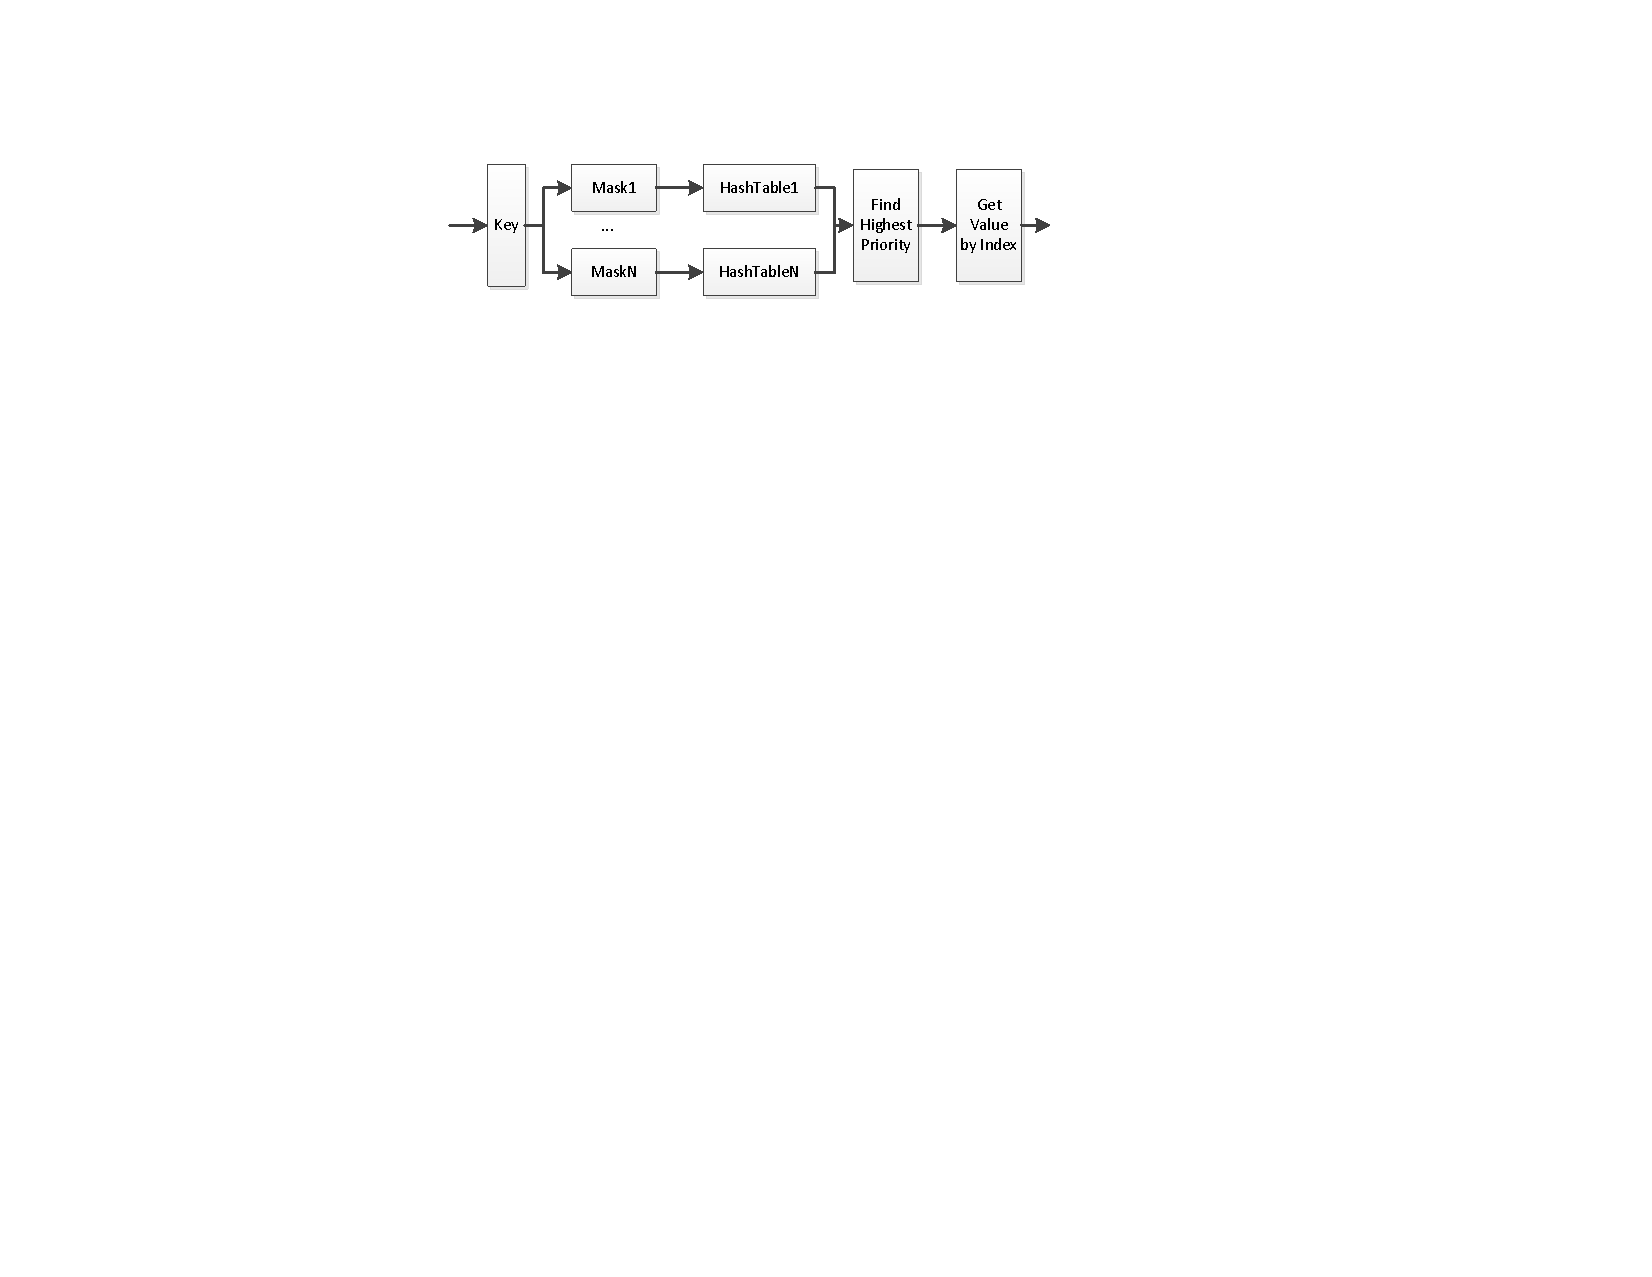
\includegraphics[width=0.8\textwidth]{image/HashTCAM}
	\caption{HashTCAM.}
	\label{clicknp:fig:hashtcam}
\end{figure}

This experiment compares the OpenFlow firewall with the Linux firewall and Click + DPDK~\cite{barbette2015fast}. For Linux, IPSet is used to handle exact match rules, while IPTable is used for wildcard rules. Also included as a reference is the performance of the Dell S6000 switch, which has limited firewall functionality and supports 1.7K wildcard rules. It is worth noting that the original Click + DPDK~\cite{barbette2015fast} does not support Receive Side Scaling (RSS). This chapter fixes this problem and finds that when using 4 cores, Click + DPDK has already achieved optimal performance. But for Linux, using as many cores as possible (up to 8 cores due to RSS limitations) can achieve optimal performance.

Figure \ref {clicknp:fig:firewall} (a) shows the packet processing rate of different firewalls with different numbers of wildcard rules. The packet size is 64B. It can be seen that both \name and S6000 can reach a maximum speed of 56.4~Mpps. Click + DPDK can reach about 18~Mpps. Since Click uses a static classification tree to implement wildcard matching, the processing speed does not change with the number of inserted rules. Linux IPTables has a low processing speed of 2.67~Mpps and the speed decreases as the number of rules increases. This is because IPTables performs linear matching for wildcard rules.

Figure \ref {clicknp:fig:firewall} (b) shows the processing latency under different loads using small packets (64B) and 8K rules. Since each firewall has significantly different capacities, the load factor is normalized to the maximum processing speed of each system. At all load levels, FPGA (\name{}) and ASIC (S6000) solutions have $\mu$s level latency (\name{} is 1.23 $\mu$s, S6000 is 0.62 $\mu$s), with very small variance ( ClickNP is 1.26 $\mu$s, for S6000 95% (percentile) is 0.63 $\mu$s). However, software solutions have larger latency and larger variance. For example, using Click + DPDK, the latency can be as high as $ 50 \mu{}s $ when the load is high. Figure \ref {clicknp:fig:firewall} (c) shows the processing latency of different packet sizes and 8K rules. With software solutions, the latency increases with the increase in packet size, mainly due to the larger memory to be copied. In contrast, FPGA and ASIC maintain the same latency, regardless of the packet size. In all experiments, the CPU usage of the \name firewall is very low (less than 5% of a single CPU core).

Finally, Figure \ref {clicknp:fig:firewall} (d) illustrates the latency of rule insertion when there are 8K rules. Click's static classification tree requires prior knowledge of all the rules, and generating a tree with 8K rules takes one minute. IPTables rule insertion takes 12 ms, which is proportional to the number of existing rules in the table. Rule insertion in Dell S6000 takes 83.7 $\mu$s. For \name{}, inserting a rule in the HashTCAM table takes 6.3 to 9.5$\mu$s for 2 to 3 PCIe round trips, while the SRAM TCAM table takes an average of 44.9 $\mu$s to update 13 lookup tables. The data plane throughput of \name does not decrease during rule insertion. The conclusion is that the \name{} firewall has similar performance to ASIC in packet processing, but has better flexibility and reconfigurability compared to ASIC.

\begin{figure*}[htbp]
	\centering
	\subfloat[]{
		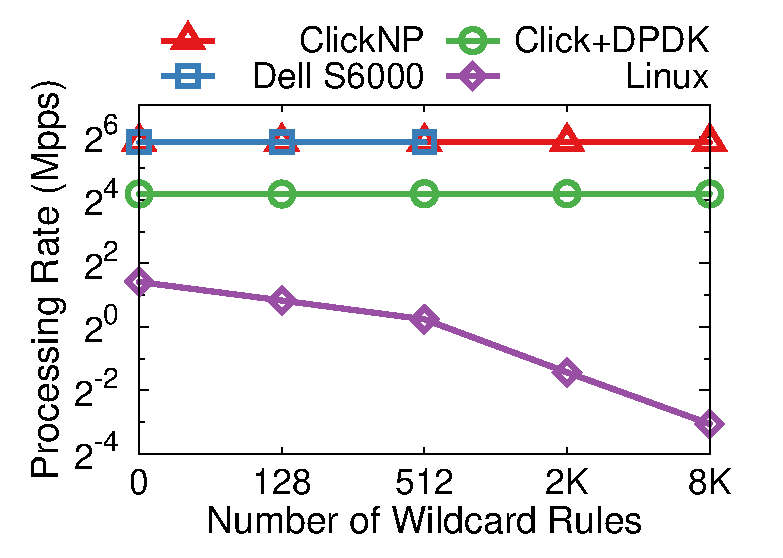
\includegraphics[width=0.5\textwidth]{eval/fw_1}
	}
	%	\subfloat[]{
	%		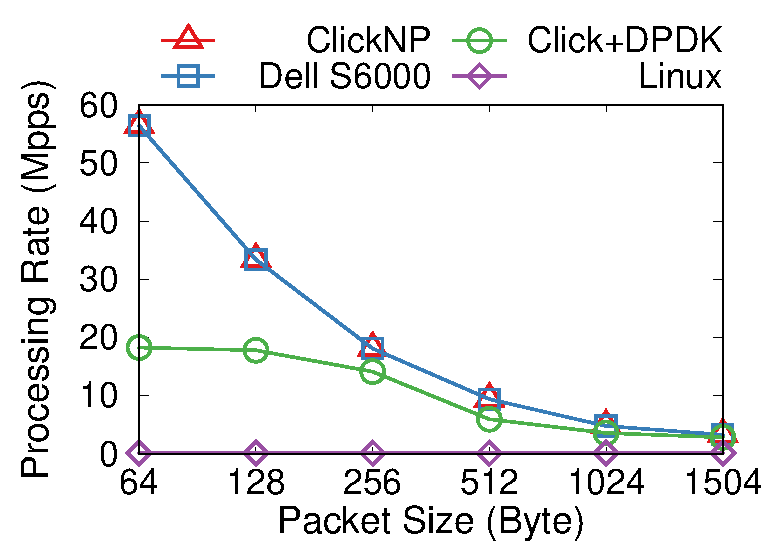
\includegraphics[width=0.225\textwidth]{eval/fw_2}
	%	}
	\subfloat[]{
		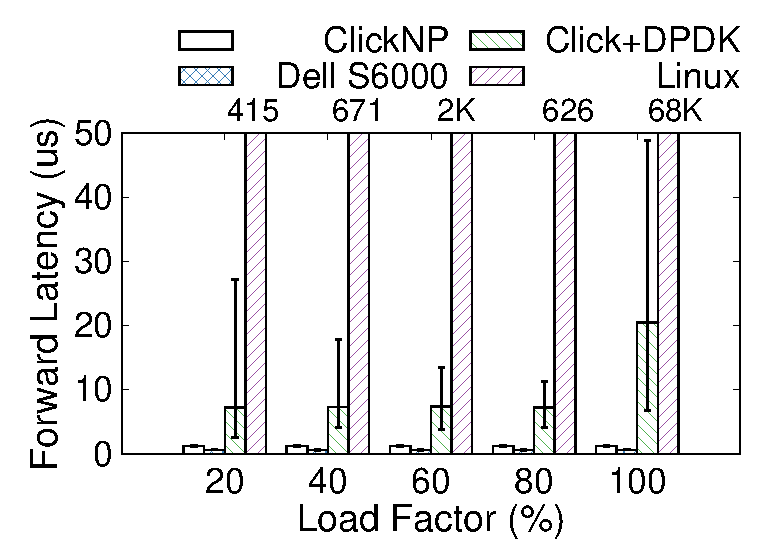
\includegraphics[width=0.5\textwidth]{eval/fw_3}
	}
	\hspace{1pt}
	\subfloat[]{
		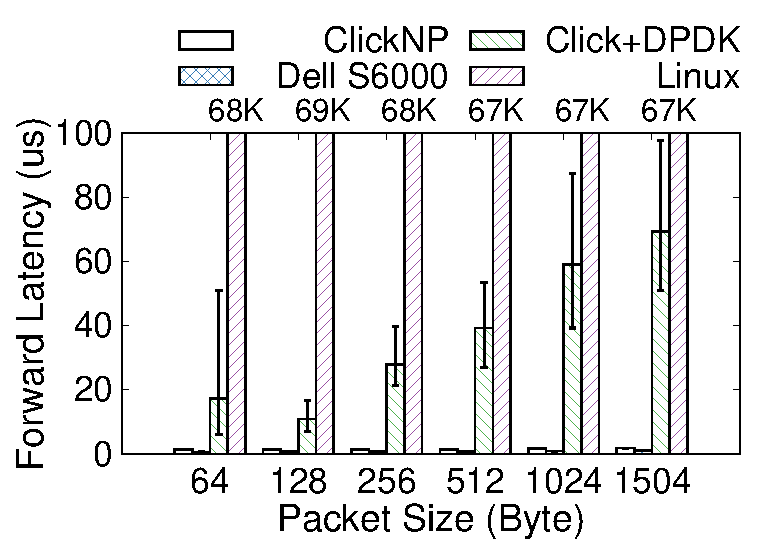
\includegraphics[width=0.5\textwidth]{eval/fw_4}
	}
	\subfloat[]{
		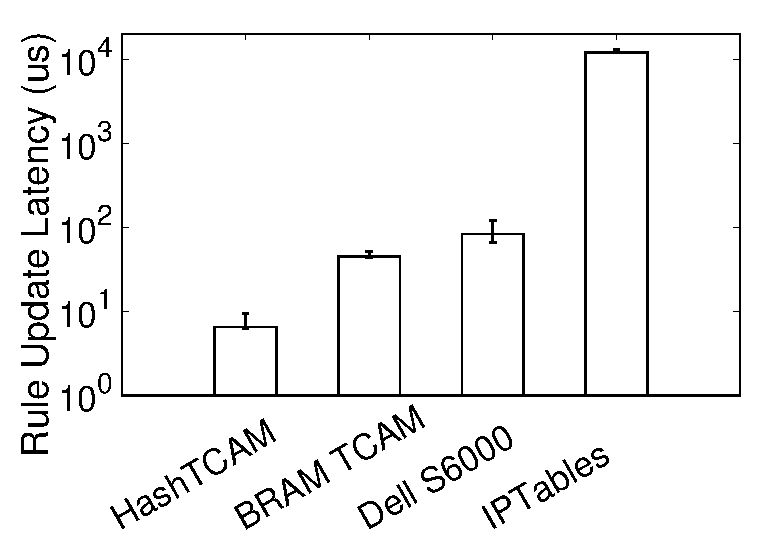
\includegraphics[width=0.5\textwidth]{eval/fw_5}
	}
	
	\caption{Firewall. The error bar represents the latency of the 5\% and 95\% percentiles. In figures (a) and (b), the packet size is 64 bytes.}
	
	\label{clicknp:fig:firewall}
\end{figure*}

\subsection{IPSec Gateway}
\label{clicknp:subsec:ipsec}

One issue with software network functions is that the CPU quickly becomes a bottleneck when packets require some computationally intensive processing, such as IPSec \cite {packetshader}. The IPSec data plane needs to use AES-256-CTR encryption and SHA-1 authentication to process IPSec packets. As shown in \S \ref {clicknp:subsec:lib}, a single AES\_CTR component can only achieve a throughput of 27.8~Gbps. Therefore, two AES\_CTR components need to run in parallel to achieve line speed. However, SHA-1 is tricky. SHA-1 divides the packet into smaller data blocks (64B). Although the computation within a data block can be pipelined, there is a dependency between consecutive blocks within an IP packet - the computation of the next block cannot start before the previous block is completed! If these data blocks are processed in sequence, the throughput will be as low as 1.07 Gbps. Fortunately, the parallelism between different packets can be utilized. Although the processing of data blocks in the current packet is still in progress, data blocks from different packets are provided. Since these two data blocks have no dependencies, they can be processed in parallel. To achieve this, we designed a new component called \textit {reservo} (short for reservation station), which can buffer up to 64 packets and schedule independent blocks for the SHA-1 component. After calculating the signature of a packet, the \textit {reservo} component sends it to the next component that attaches the SHA-1 HMAC to the packet.

There is another intricate issue. Although the SHA-1 component has a fixed delay, the total delay of the packets varies, that is, it is proportional to the size of the packet. When scheduling multiple packets in the SHA-1 calculation, these packets may be rearranged, for instance, smaller packets behind a large packet may be completed earlier. To ensure the output packets maintain the same order as the input, a \textit{reorder buffer} component is further added after the SHA-1 component, which stores out-of-order packets and restores the original order according to the sequence number of the packets. Figure \ref{clicknp:fig:IPSec-arch} illustrates the component structure of the IPSec gateway.

\begin{figure}[htbp]
	\centering
	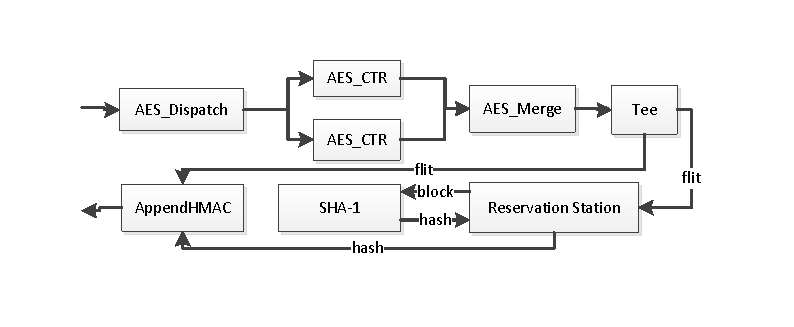
\includegraphics[width=0.8\textwidth]{image/IPSec}
	\caption{Component architecture of the IPSec gateway.}
	\label{clicknp:fig:IPSec-arch}
\end{figure}

The following compares the IPSec gateway and StrongSwan~\cite{strongswan}, using the same cipher suite AES-256-CTR and SHA1. In the case of a single IPSec tunnel, Figure \ref{clicknp:fig:IPSec}(a) displays the throughput of different packet sizes. For all scales, IPSecGW achieves line rate, that is, 64B packets are 28.8 Gbps, and 1500B packets are 37.8 Gbps. However, StrongSwan can only reach up to 628 Mbps, and as the packet size decreases, the throughput will also decrease. This is because the smaller the size, the more packets need to be processed, so the system needs to calculate more SHA1 signatures. Figure \ref{clicknp:fig:IPSec}(b) shows the latency under different load factors. Similarly, the constant delay produced by IPSecGW is 13 $\mu$s, but StrongSwan will produce a larger delay and higher variance, up to 5 ms!

\begin{figure*}[htbp]
	\centering
	\subfloat[]{
		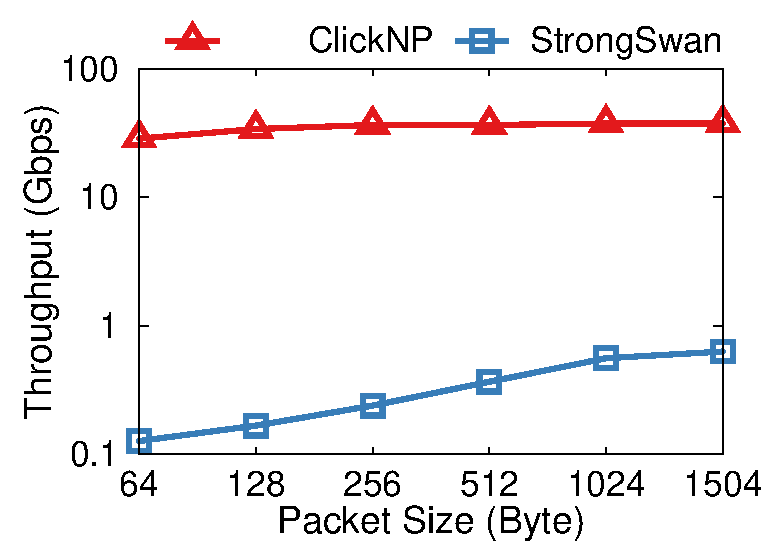
\includegraphics[width=0.5\textwidth]{eval/ipsec_1}
	}
	\subfloat[]{
		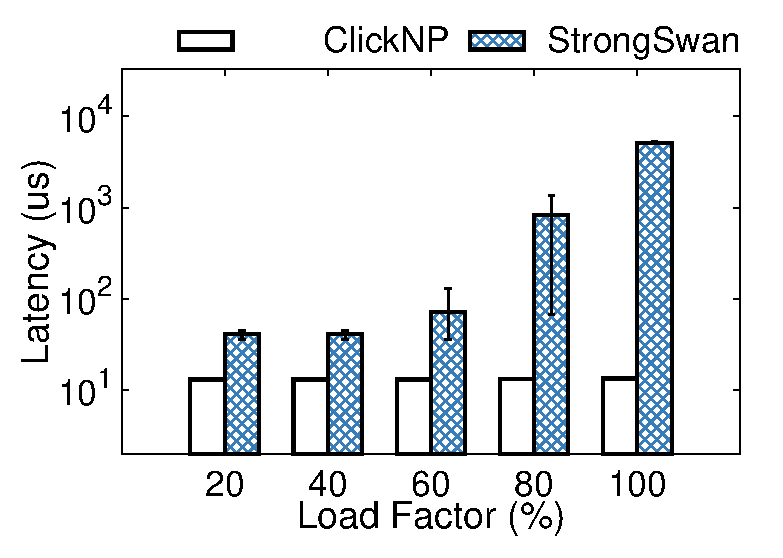
\includegraphics[width=0.5\textwidth]{eval/ipsec_2}
	}
	
	\caption{IPSec gateway.}
	
	\label{clicknp:fig:IPSec}
\end{figure*}

\subsection{L4 Load Balancer}
The L4 load balancer is implemented according to the \textit{multiplexer} (MUX) in Ananta~\cite{ananta}. The MUX server essentially examines the packet header and checks whether a \textit{direct address} (DIP) has been allocated for this stream. If so, the packet is forwarded to the server indicated by the DIP through the NVGRE tunnel. Otherwise, the MUX server will call the local controller to allocate a DIP for the stream. The MUX server needs to maintain the state by stream. Since there are failures and the backend server list needs to be updated in real time to avoid black holes, hash-based ECMP cannot be used. In addition, advanced LB may also require load-aware balancing. The flow table is used to record the mapping of the flow to its DIP. To handle the large traffic in the data center, it requires the L4LB to support up to 32 million streams in the flow table. Clearly, such a large flow table cannot fit into the FPGA's BRAM and must be stored in the onboard DDR memory. However, accessing DDR memory is slow. To improve performance, a 4-way associative flow cache with 16K cache lines is created in the BRAM. The least recently used (LRU) algorithm is used to replace entries in the flow cache.

As depicted in Figure \ref{clicknp:fig:L4LB}, the incoming packet initially traverses a \textit{parser} component, which extracts the 5-tuple and transmits them to the \textit{flow cache} component. If the flow is not located in the flow cache, the packet's metadata is forwarded to the global flow table, which reads the complete table in the DDR. If there is still no matching entry, then this packet is the first packet of the flow, and the request is dispatched to the \textit{DIPAlloc} component to allocate a DIP for this flow according to the load balancing policy. After the DIP is determined, an entry is inserted into the flow table.

Upon determining the DIP of the packet, the encapsulation component will retrieve the next hop information, such as the IP address and VNET ID, and generate the packet of the NVGRE encapsulation accordingly. For the remaining packets of the flow, the DIP is extracted from the flow state. If a FIN packet is received or a timeout occurs, the flow entry will be invalidated before receiving any new packets from the flow. After determining the DIP, the next hop metadata is retrieved from the BRAM and the NVGRE header is encapsulated to guide the packet to the allocated DIP.

Except for the \textit{DIPAlloc} component, all components are placed in the FPGA. Since only the first packet of the flow may encounter \textit{DIPAlloc} and the allocation policy may also be complex, it is more suitable to run the \textit{DIPAlloc} on the CPU, which is another example of joint CPU-FPGA processing.

\begin{figure}[htbp]
	\centering
	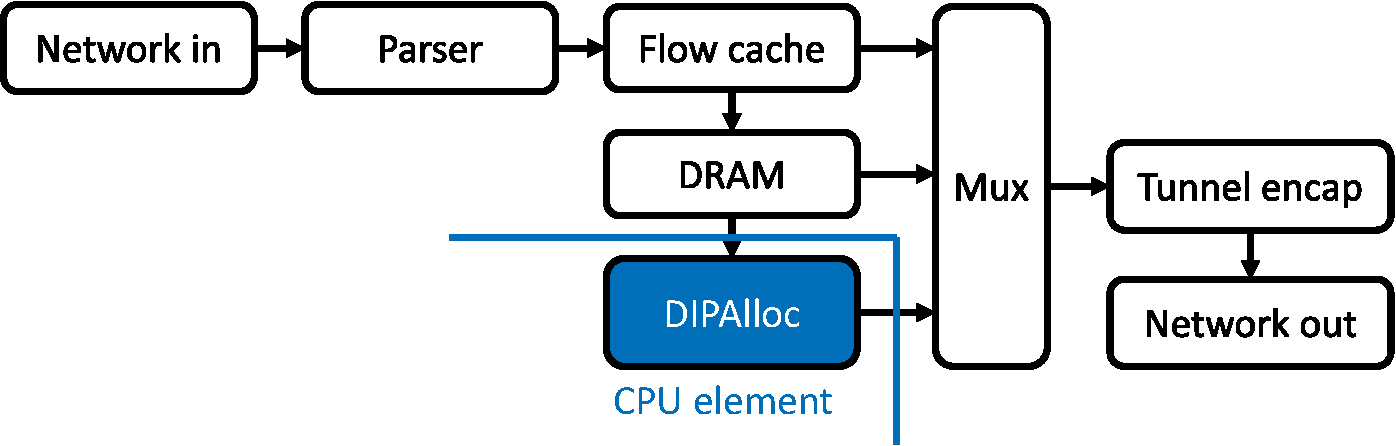
\includegraphics[width=0.8\textwidth]{image/L4LoadBalancer}
	\caption{Component architecture of the L4 load balancer.}
	\label{clicknp:fig:L4LB}
\end{figure}

The following compares L4LB with Linux Virtual Server (LVS) \cite {lvs}.
To stress test the system, a large number of concurrent UDP streams are generated using 64B packets, targeting a Virtual IP (VIP).
Figure \ref {clicknp:fig:l4} (a) shows the processing rate with different numbers of concurrent streams.
When the concurrent traffic is less than 8K, L4LB reaches a line rate of 51.2Mpps.
However, as the number of concurrent streams increases, the processing rate begins to decline.
This is due to cache misses in the flow cache of L4LB.
When a flow is missing from the flow cache, L4LB must access the onboard DDR memory,
which leads to a performance drop.
When the traffic is too high, for example, 32M, cache misses dominate and for most packets,
L4LB needs to access DDR memory once. Therefore the processing speed drops to 11Mpps.
In any case, the processing rate of LVS is very low.
Since LVS associates the VIP with only one CPU core, its processing rate must reach 200Kpps.

The translation of your LaTeX content into English while preserving the original LaTeX markup structure is as follows:

\begin{figure*}[htbp]
	\centering
	
	\subfloat[]{
		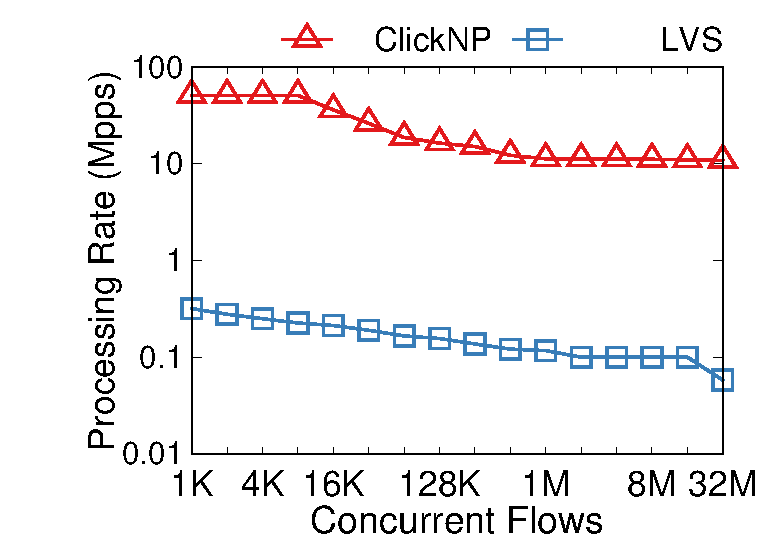
\includegraphics[width=0.5\textwidth]{eval/l4_2}
	}
	\subfloat[]{
		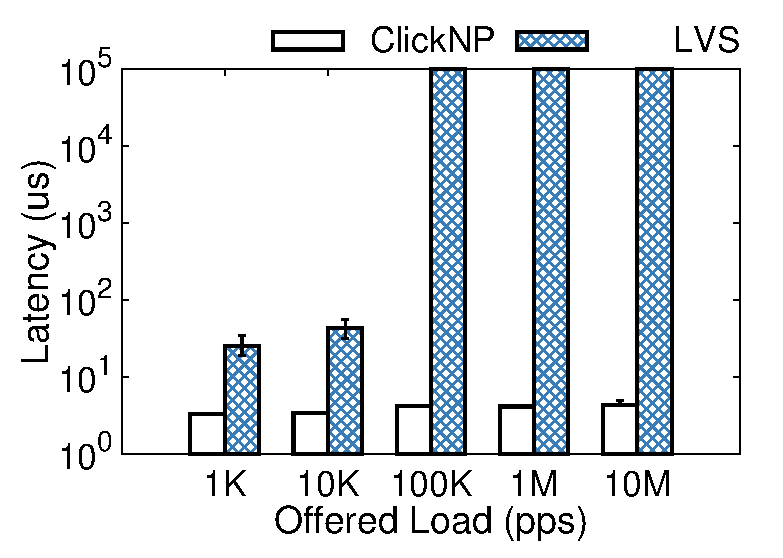
\includegraphics[width=0.5\textwidth]{eval/l4_1}
	}
	
	\subfloat[]{
		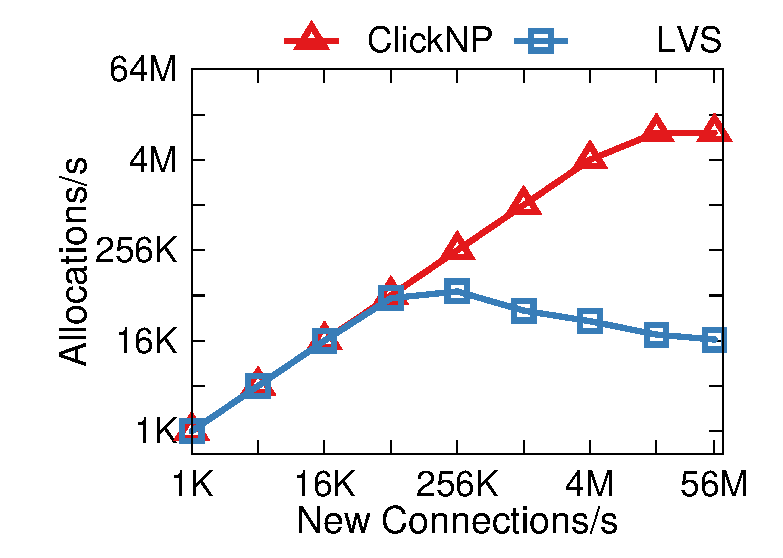
\includegraphics[width=0.5\textwidth]{eval/l4_3}
	}
	
	\caption{Performance evaluation of L4 load balancer.}
	\label{clicknp:fig:l4}
	
\end{figure*}

Figure \ref {clicknp:fig:l4} (b) illustrates the latency under varying load conditions.
In this experiment, the number of concurrent streams is held constant at one million.
It is evident that L4LB achieves an impressively low latency of 4 $\mu$s.
However, LVS incurs a delay of approximately 50 $\mu$s.
When the throughput load exceeds 100Kpps, the queuing delay escalates rapidly, surpassing the processing capacity of LVS.

Lastly, Figure \ref {clicknp:fig:l4} (c) contrasts the capacity of L4LB and LVS to accept new flows.
This experiment directs PktGen to generate as many single-packet micro-flows as possible.
It is observable that L4LB can accommodate up to 10M new connections per second.
Given that a single PCIe slot can transmit 16.5M data per second, the bottleneck remains DDR access.
For simplicity, the \textit {DIPAlloc} component in this paper allocates DIP in a round-robin fashion.
For complex allocation algorithms, the CPU core of \textit {DIPAlloc} will become the bottleneck, and performance can be enhanced by replicating the \textit {DIPAlloc} component on more CPU cores.
For LVS, due to its limited packet processing capacity, it can accept a maximum of 75K new connections per second.

\subsection{pFabric Flow Scheduler}

\name is also a valuable tool for network research.
Owing to its flexibility and high performance, \name can swiftly create prototypes of the latest research and apply them to real environments.

This section employs \name to implement a recently proposed packet scheduling rule--pFabric \cite {pfabric}.
pFabric scheduling is straightforward. It maintains a shallow buffer (32 packets) and always dequeues the packet with the highest priority. When the buffer is full, the packet with the lowest priority will be discarded.
pFabric has achieved near-optimal flow completion time in data centers.
In the original paper, the authors proposed using a Binary Comparison Tree (BCT) to select the packet with the highest priority.
However, although BCT only requires $O(log_2 N)$ cycles to calculate the packet with the highest priority, there is a dependency between two consecutive selection processes. This is because only after the previous selection is completed can the packet with the highest priority be known, and then the next selection process can be reliably started.
This restriction requires a clock frequency of at least 300MHz to achieve a line speed of 40Gbps, which is currently unattainable for the existing FPGA platform.

\begin{figure}[htbp]
	\centering
	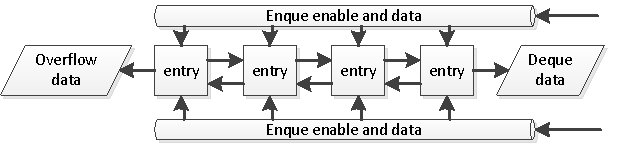
\includegraphics[width=0.8\textwidth]{image/PriorityQueue}
	\caption{Shift register priority queue.}
	\label{clicknp:fig:ShiftRegPrioQueue}
\end{figure}

This paper employs a distinct method to implement the pFabric scheduler, which is more amenable to parallelization.
The approach is grounded on the \textit{shift register priority queue} \cite {moon2000scalable}.
As depicted in Figure \ref{clicknp:fig:ShiftRegPrioQueue}, entries are stored in $K$ registers in a non-increasing priority order.
During dequeuing, all entries shift to the right and are popped from the head. This process only necessitates 1 cycle.
For the enqueue operation, the metadata of the new packet will be forwarded to all entries.
At this point, for each entry, a local comparison can be conducted between the packet in the entry, the new packet, and the packet in the adjacent entry.
Given that all local comparisons can be executed in parallel, the enqueue operation can also be accomplished in 1 cycle.
Enqueue and dequeue operations can be further parallelized.
Hence, a packet can be processed in a single cycle.
Figure \ref{clicknp:fig:pfabric-arch} illustrates the component architecture of the pFabric flow scheduler.

\begin{figure}[htbp]
	\centering
	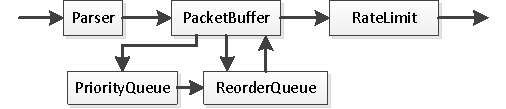
\includegraphics[width=0.8\textwidth]{image/PFabric}
	\caption{Component architecture of pFabric flow scheduler.}
	\label{clicknp:fig:pfabric-arch}
\end{figure}

In this experiment, a software TCP flow generator\cite {mqecn} was modified to embed the flow priority, that is, the total size of the flow, into the packet payload. The experiment generated flows in accordance with the data mining workload in \cite {pfabric} and utilized the \textit {RateLimit} element to further set the exit port limit to 10~Gbps. The pFabric application schedules the traffic in the exit buffer based on the flow priority. Figure \ref{clicknp:fig:pfabric} presents the average flow completion time (FCT) and ideal value of pFabric and TCP with a Droptail queue. This experiment validates that pFabric achieves near-optimal FCT in this straightforward scenario.

\begin{figure}[htbp]
	\centering
	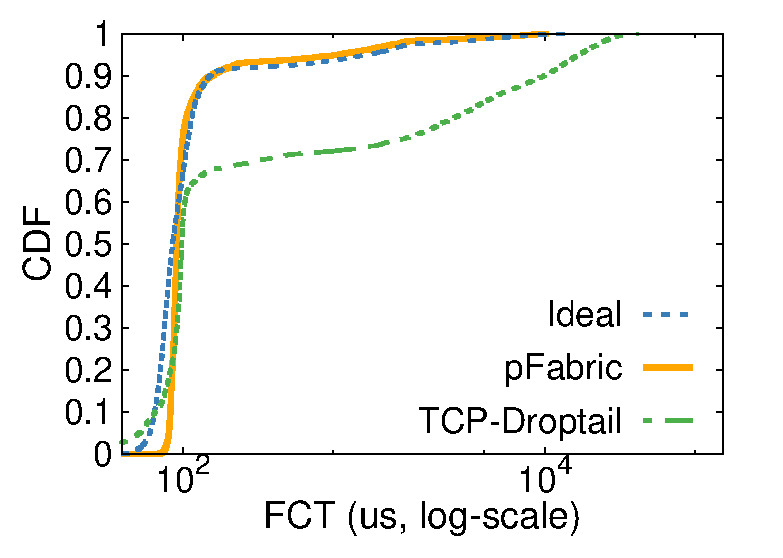
\includegraphics[width=0.6\textwidth]{eval/pfabric}
	\caption{Verification of pFabric.}
	\label{clicknp:fig:pfabric}
\end{figure}

\subsection{Fault-tolerant EPC SPGW}

The data plane of the LTE core network (EPC) employs S-GW and P-GW to process network packets, with its processing flow resembling that of the IPSec gateway, as depicted in Figure \ref{clicknp:fig:epc-arch}. The EPC SPGW must maintain the state for each bearer (i.e., user), with the bearer's state being modified each time a packet passes through. The EPC SPGW demands not only high throughput and low latency, but also high fault tolerance, meaning that hardware failures should be imperceptible to users and the state should not be lost.

\begin{figure}[htbp]
	\centering
	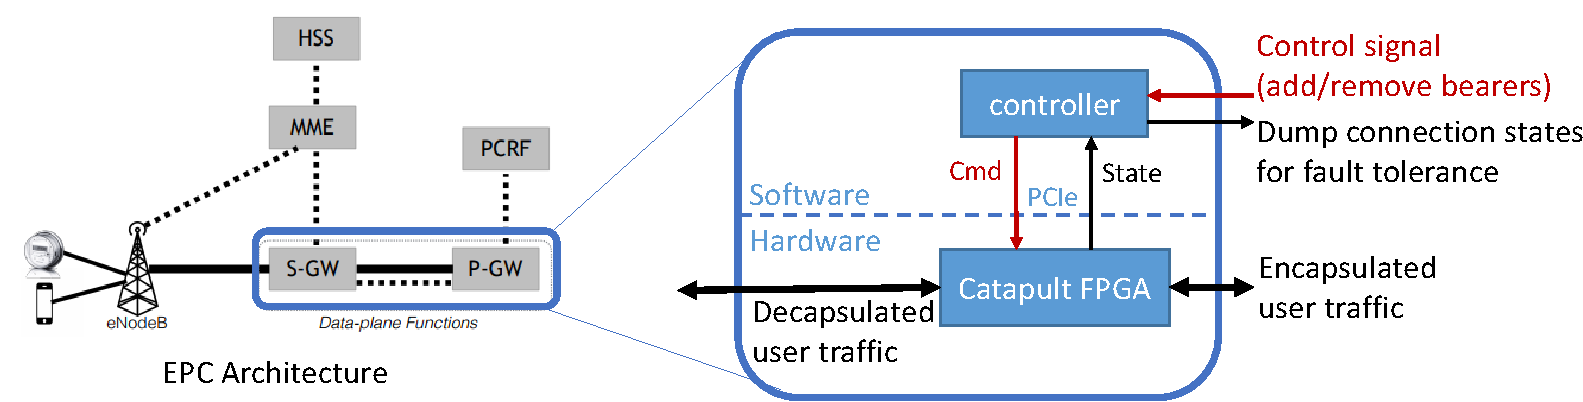
\includegraphics[width=1.0\textwidth]{image/EPC_arch}
	\caption{Acceleration architecture of LTE core network (EPC).}
	\label{clicknp:fig:epc-arch}
\end{figure}

High fault tolerance is achieved using the state machine replication method outlined in Section \ref{subsec:clicknp:fault-tolerance}, as illustrated in the component structure in Figure \ref{clicknp:fig:epc-element}. Each user requires approximately 300 bytes of state, the FPGA's on-chip memory can cache the state of around 4K users, and the on-board BRAM can store the state of 10M users, thus a single FPGA can support up to 10M concurrent connections. In the typical scenario where user access follows a power law distribution, the FPGA's throughput can reach 40 M packets per second (pps); in the worst-case scenario, due to cache misses, the throughput can reach 20 M pps. Under normal circumstances, the FPGA's 95\% latency is 4 $\mu$s. The control plane is implemented through the PCIe I/O pipeline, with a 95\% control plane latency of 1 $\mu$s and a throughput of 1M add or delete user operations per second. When adding a new backup node, it is necessary to back up the user state of the original node to the new node. When the network is idle, this state migration process can fully utilize the 40 Gbps bandwidth, and state replication can be achieved in just 0.8 seconds.

\begin{figure}[htbp]
	\centering
	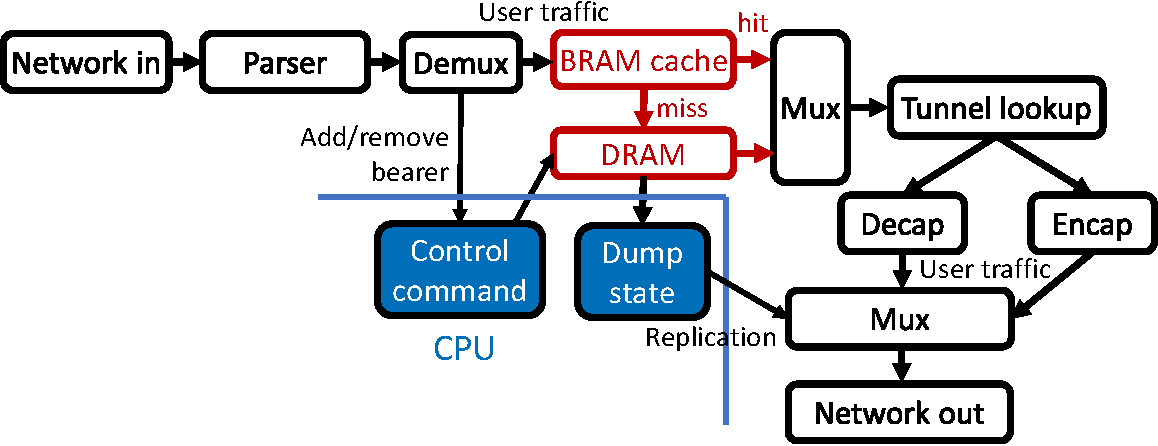
\includegraphics[width=1.0\textwidth]{image/EPC_element}
	\caption{Component structure of LTE SPGW.}
	\label{clicknp:fig:epc-element}
\end{figure}

\section{Discussion: Resource Utilization}

\egg{
	To assess the area cost overhead of ClickNP in comparison to a hand-written hardware description language, we implemented several ClickNP elements that resemble network functions in NetFPGA 10G \cite{netfpga} reference router and Openflow switch projects.
	Table \ref{clicknp:tab:netfpga} compares the relative area cost of ClickNP over NetFPGA using Vivado high-level synthesis 2015.4 and Altera OpenCL 15.1.
	Most ClickNP implementations exhibit less than 100\% logic overhead and less than 30\% BRAM overhead. For smaller elements (\eg IP checksum), a fixed element overhead is predominant.
}

This section will evaluate the resource utilization of the \name network function. The results are summarized in Table \ref {clicknp:tab:applications}. Except for the IPSec gateway that utilizes most of the BRAM to store the code book, all other network functions only use a moderate amount of resources (5 to 50%), leaving room for more network functions.

\begin{table}[htbp]
	\centering
	\caption{Summary of ClickNP network functions.}
	\label{clicknp:tab:applications}
	\small
	\begin{tabular}{l|r|r|r|r}
		\toprule
		Network Function & LoC$^\dagger$ & \#Elements & LE & BRAM \\
		\midrule
		\egg{
			Pkt generator & 13 & 6 & 16\% & 12\% \\
			Pkt capture & 12 & 10 & 8\% & 5\% \\
			OpenFlow firewall & 23 & 7 & 32\% & 54\% \\
			IPSec gateway & 37 & 10 & 35\% & 74\% \\
			L4 load balancer & 42 & 13 & 36\% & 38\% \\
			pFabric scheduler & 23 & 7 & 11\% & 15\% \\
		}
		Pkt generator & 665 & 6 & 16\% & 12\% \\
		Pkt capture & 250 & 11 & 8\% & 5\% \\
		OpenFlow firewall & 538 & 7 & 32\% & 54\% \\
		IPSec gateway & 695 & 10 & 35\% & 74\% \\
		L4 load balancer & 860 & 13 & 36\% & 38\% \\
		pFabric scheduler & 584 & 7 & 11\% & 15\% \\
		\bottomrule
		\multicolumn{5}{l}{$^\dagger$ The sum of the number of lines of code for all component description languages and configuration files.}
	\end{tabular}
\end{table}

Next, we examine the overhead of \name's fine-grained modularization. Since each component will generate logic block boundaries and only use FIFO buffers to communicate with other blocks, there should be overhead. To measure this overhead, create a simple "\textit{empty}" component that only passes data from one input port to the output port. The resource utilization of this \textit{empty} component can well reflect the overhead of modularization. Different high-level synthesis tools may use different amounts of resources, but they are all very low, with a minimum of 0.15% and a maximum of 0.4%. Therefore, the overhead introduced by fine-grained modularization is small. Future work can also explore the fusion of adjacent components in the computation flow graph to further reduce the modularization overhead of components.

Finally, we examine the efficiency of the hardware description language code generated by \name in comparison to manually written hardware description language. For this, we use NetFPGA \cite {netfpga} as a reference. Initially, we extract the key modules in NetFPGA, which have been optimized by experienced Verilog programmers, and implement corresponding components with the same functionality in \name. Subsequently, using different high-level synthesis tools as the backend, we compare the relative area cost between these two implementations. The results are summarized in Table \ref {clicknp:tab:netfpga}. As different tools may have varying area costs, we record the maximum and minimum values. It is evident that the automatically generated hardware description language code uses more area compared to manually optimized code. However, the difference is not substantial. For complex modules (as shown at the top of the table), the relative area cost is less than twice. For smaller modules (as shown at the bottom of the table), the relative area cost appears larger, but the absolute resource usage is minimal. This is because existing high-level synthesis tools generate fixed control logic for each component, resulting in area overhead.

\begin{table}[htbp]
	\centering
	\caption{Area overhead compared to NetFPGA.}
	\label{clicknp:tab:netfpga}
	\small
		\begin{tabular}{l|r|r|r}
			\toprule
			\multirow{2}{2.2cm}{NetFPGA Function} & Logic Lookup Table (LUT) & Register & Memory (BRAM) \\
			& Min / Max & Min / Max & Min / Max \\
			\midrule
			Input selector  & 2.1x / 3.4x & 1.8x / 2.8x & 0.9x / 1.3x \\
			Output queue   & 1.4x / 2.0x & 2.0x / 3.2x & 0.9x / 1.2x \\
			Packet header parser  & 0.9x / 3.2x & 2.1x / 3.2x & N/A \\
			Openflow lookup table & 0.9x / 1.6x & 1.6x / 2.3x & 1.1x / 1.2x \\
			\midrule
			\midrule
			IP checksum calculation    & 4.3x / 12.1x & 9.7x / 32.5x & N/A \\
			Tunnel encapsulation          & 0.9x / 5.2x & 1.1x / 10.3x & N/A \\
			\bottomrule
		\end{tabular}
\end{table}

In conclusion, \name can generate efficient hardware description language for FPGA with only a moderate area cost, and can construct practical network functions. Looking ahead, FPGA technology is still rapidly evolving. For instance, the area of Intel's Arria 10 FPGA and the latest Stratix 10 FPGA are 2.5 times and 10 times that of the chip used in this study (Stratix V), respectively. Therefore, the area cost of high-level synthesis will become less significant in the future.

\section{Extension: Computation-Intensive Applications}

Some network functions are computation-intensive, such as the IPSec gateway in Section \ref{clicknp:subsec:ipsec} which needs to encrypt and sign the content of each data packet. Due to the large amount of computation for a data packet, the area of fully unfolding the entire computation flow graph into a pipeline will exceed the capacity of the FPGA. Therefore, it is necessary to \emph{exchange time for space}, and split the computation flow graph. Due to the dependencies in the computation process, Section \ref{clicknp:subsec:ipsec} shows how to use \emph{reservation stations} to divide the computation of data packets into multiple stages, save intermediate states, and fully utilize the parallelism between different connections. This section discusses two applications with larger computations: HTTPS RSA acceleration and neural network inference, to demonstrate the general method of implementing computation-intensive applications.

\subsection{HTTPS RSA Acceleration}

HTTPS is a protocol for secure connections with web services. With increasing user concern for privacy, more and more web services provide access through HTTPS. Since 2010, the proportion of HTTPS traffic has grown by 40% every six months, and by 2016 it accounted for over 40% of all network connections.

HTTPS provides three mechanisms to ensure security. First, when a connection is established, it uses to verify the identity of the web server and create a shared key for both parties. Second, it encrypts the data transmission between the user and the web server. Third, it checks the integrity of the data. Among these three mechanisms, connection establishment is the most computation-intensive part because it requires asymmetric key operations (such as the RSA algorithm).

Without enabling HTTPS, a single CPU core can process over 7,000 HTTP requests per second. When using HTTPS, the throughput drops to 1/35 due to the TLS handshake in the connection setup. The high computational overhead of the TLS handshake has always been a major obstacle for high-traffic websites to deploy HTTPS to ensure security.

In the TLS handshake, the web server carries out decryption using the RSA private key. As depicted in Figure \ref{clicknp:fig:https-accelerator}, RSA decryption is mathematically a large integer power modulus operation, where the base, exponent, and modulus are all large integers. By binary decomposition of the exponent, the large integer power modulus operation can be implemented by iteratively performing multiple multiplication modulus operations. The multiplication modulus operation can be transformed into 3 multiplication, 1 addition, and 1 subtraction operations by the Montgomery algorithm. For a 2048-bit private key, decryption requires approximately 8 million 16-bit integer multiplication operations. Although TLS certificate parsing and protocol processing are also complex, the number of computations required is significantly less than decryption. Therefore, we modify the OpenSSL library to offload RSA decryption operations to the FPGA and retain the other parts on the CPU.

Clearly, fully unfolding the entire RSA decryption process into digital logic would occupy too much chip area, so it is necessary to trade time for space and construct a smaller scale multiplication and addition array, repeating the computation multiple times. For a 2048-bit key, even the innermost 1024-bit large integer multiplier has already exceeded the FPGA's DSP quantity limit, so it is necessary to further divide the large integer multiplication. In the Montgomery algorithm, the 3 multiplications can obviously reuse the same multiplier array.\footnote{If three separate multiplier arrays are used, then under the condition of a fixed total area, the parallelism of each multiplier array will become 1/3, and since there is data dependency between the 3 multiplications, the delay of the RSA decryption operation will increase to about 3 times. Therefore, when the parallelism is adjustable, in most cases it is beneficial to combine multiple elements that cannot be executed in parallel into one element with greater parallelism.} The ModMulti controller in Figure \ref{clicknp:fig:https-accelerator} moves data between the multiplier, adder, and subtractor; the Binary Exp controller moves data between multiple ModMulti operations. In addition, since there is pipeline delay in the operation components, and there is dependency between the computations of a single RSA decryption, many operation components will be idle if only one RSA decryption is performed. In order to fully utilize the parallelism of the FPGA, multiple RSA decryption tasks need to be processed concurrently. The ModMulti and Binary Exp controllers need to manage the intermediate data and execution status of concurrent tasks, and schedule unrelated subtasks to the computation components.

\begin{figure}[htbp]
	\centering
	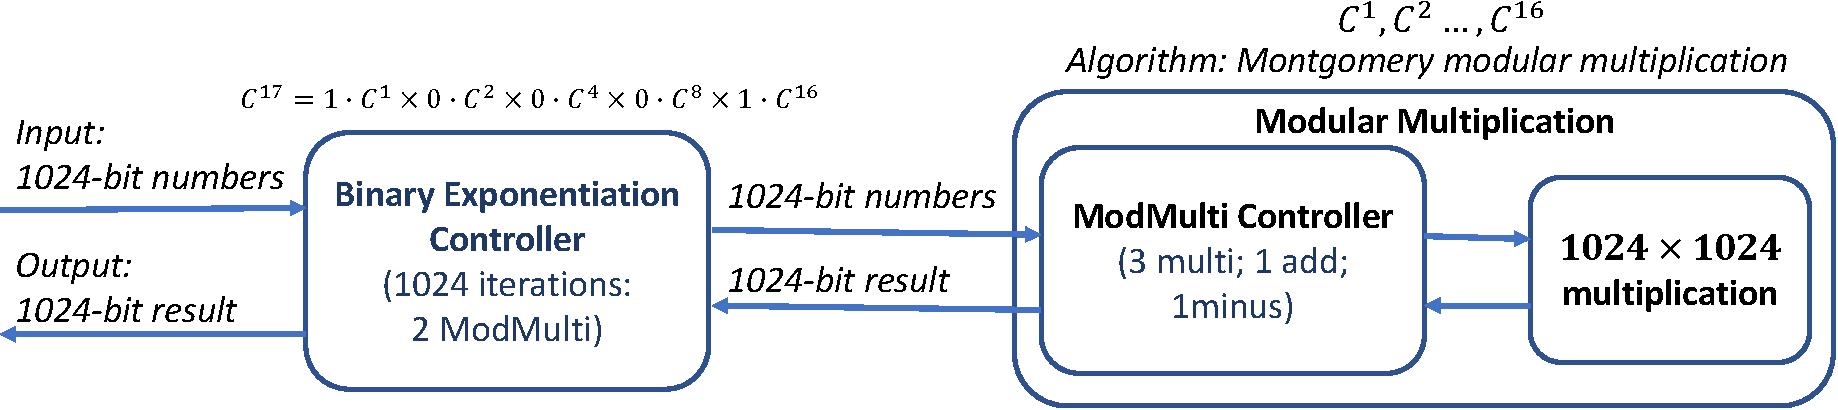
\includegraphics[width=1.0\textwidth]{image/https_accelerator}
	\caption{Component structure of the HTTPS accelerator (simplified diagram).}
	\label{clicknp:fig:https-accelerator}
\end{figure}

Clearly, manually implementing the logic of controller cache management, task division, concurrency control, data movement, etc. is quite laborious. For this reason, we aim to automatically generate controller code from the source code shown in Figure \ref{clicknp:fig:rsa-code}.

\begin{figure}[t!]
	\renewcommand{\baselinestretch}{0.7}
	\small
	\centering
	\begin{tabular}{c}
\begin{lstlisting}
template<T> uint##(T*2) Karatsuba(uint##T a, b) {
    if (T > 256) { // karatsuba multiplication
        const T' = T/2;
        uint##T' a0 = a[T-1:T'], a1 = a[T'-1:0];
        uint##T' b0 = b[T-1:T'], b1 = b[T'-1:0];
        uint##T m0 = Karatsuba<T'>(a0, b0);
        uint##T m1 = Karatsuba<T'>(a1, b1);
        uint##T m2 = Karatsuba<T'>(a0 + a1, b0 + b1);
        return (m0 << T) + ((m2 - m0 - m1) << T') + m1;
    }
    else { // simple school book multiplication
        uint32 t[T*2/16];
        for (i=0; i<T; i+=16)
            for (j=0; j<T; j+=16)
                t[(i + j) / 16] += a[i+15:i] * b[j+15:j];
        uint##(T*2) result;
        for (i=0; i<T*2; i+=16) {
            t[i+1] += t[i][31:16];
            result[i+15:i] = t[i][15:0];
        }
    }
}
uint1024 ModMulti(uint1024 a, b, m, m') {
    uint2048 t = Karatsuba<1024>(a, b);
    uint1024 n = Karatsuba<1024>(t[1023:0], m')[1023:0];
    uint2048 sum = Add<2048>(t, Karatsuba<1024>(m * n));
    uint1024 s = sum[2047:1024];
    int1024 diff = Subtract<1024>(s, n);
    return IsPositive<1024>(diff) ? diff : s;
}
uint1024 ModExp(uint1024 a, e, m, m') {
    uint1024 square = a, result = 1;
    for (i = 0; i < 1024; i++) {
        if (e[i])
            result = ModMulti(result, square, m);
        square = ModMulti(square, square, m);
    }
    return result;
}
\end{lstlisting}
	\end{tabular}
	\caption{Schematic code of \name for large integer power modulus operation used in 2048-bit RSA decryption. The \name template is a syntactic sugar for generating recursive structure code, which will be expanded and eliminate invalid code at compile time. Functions not declared as inline are implemented as independent components, just like the \texttt{async} primitive.}
	\label{clicknp:fig:rsa-code}
\end{figure}

Firstly, \name begins from the innermost loop, attempting to unroll as many loop layers as possible to parallelize the maximum number of computations. In instances of multiple parallel loops (such as the multiplication and addition in Figure \ref{clicknp:fig:rsa-code}), the unroll count for each loop needs to correspond to the number of computations \footnote{For instance, if two loops have 512 and 1024 iterations respectively, the ratio of the unroll count for the two loops is 1:2.}, ensuring that the throughput of each computation module is matched. Developers can specify the unroll count for each loop separately; for programs where the loop iteration count is statically known at compile time, a global unroll count can also be specified as the unroll count for the loop with the highest computational intensity, and \name will automatically match the unroll count for other loops.\footnote{For programs with uncertain loop times, developers can manually divide them into several static areas and specify the required throughput or area target for each area.} The upper limit of the loop unroll count is dependent on the FPGA's hardware capacity, and developers can configure it based on the resource estimates reported by the high-level synthesis tool or the results after synthesis and layout routing. Some programs have multi-layer loops whose order can be interchanged, and the data locality of the code generated by splitting different loop levels varies, resulting in different amounts of required data movement. When writing \name code, developers should place the loop with the highest parallelism and strongest data locality in the innermost layer, so that when the compiler unrolls the inner loop, it can minimize the data movement overhead.

Next, \name generates controller code. To generate code for concurrent execution with hidden latency, \name compiles the computation components (i.e., unrolled loops) and the code for data movement between on-chip memory and computation components using high-level synthesis tools, to calculate their latency and throughput. The number of tasks executed concurrently is the product of latency and throughput. The controller stores the current execution status and intermediate data of each task in the on-chip memory and schedules the split sub-computation tasks to the computation components.

A typical inference neural network comprises several sparse and dense layers. Sparse layers primarily read randomly from larger feature arrays, while dense layers mainly perform matrix or vector multiplication. Each sparse and dense layer is represented by a \name component, and the computation flow graph of the neural network is the connection between \name components. If each component is implemented as separate hardware logic, the on-chip resources will be fragmented. For a specific task, only a few computation components are running at the same time, resulting in longer latency for a single task. Therefore, it is necessary to extract common computation components from different components. For network functions, \name has difficulty optimizing this because the types of computations performed by various components of network functions are different and it is difficult to extract common parts.

The method to extract common computation components is to compare the isomorphism of loops in different components, that is, whether the abstract syntax trees of two loops can be made completely the same by replacing the accessed array names and loop variable names. If the loops in several different components are isomorphic, these refactored loops can be extracted into a new \texttt{async} component. For example, access to global memory in each sparse layer can be extracted into one component, matrix and vector multiplication in each dense layer can be extracted into one component, and the relu activation function in each dense layer can be extracted into another component. Next, similar to RSA decryption, \name unrolls the inner loops as much as possible and generates controller code. As shown in Figure \ref{clicknp:tab:neural-network}, the higher the parallelism of loop unrolling, the lower the latency of neural network inference.

\begin{table}[htbp]
	\centering
	\caption{Latency of neural network inference at different parallelism levels of dense layers. The neural network used consists of three sparse layers and four dense layers. The features obtained by the three parallel-executing sparse layers are concatenated with other input features and then enter the dense layers. The four dense layers form a pipeline, each consisting of matrix and vector multiplication, activation function, and normalization function.}
	\label{clicknp:tab:neural-network}
	\small
	\begin{tabular}{l|r}
		\toprule
		Dense layer parallelism & Per-sample latency ($\mu$s) \\
		\midrule
		8 & 188.2 \\
		16 & 98.2 \\
		32 & 49.3 \\
		64 & 26.1 \\
		128 & 17.5 \\
		256 & Insufficient resources \\
		\bottomrule
	\end{tabular}
\end{table}

Finally, it should be noted that for compute-intensive tasks, although the high-level synthesis method adopted by \name significantly improves the development efficiency compared to manually writing low-level FPGA code, its area overhead may be considerably higher than manually optimized FPGA code. Fortunately, the performance of network packet processing tasks is primarily limited by network bandwidth, and in most cases, the FPGA area is not a significant consideration.

\egg{
	\textbf{Stateful L4 load balancer.} We compare our ClickNP implementation with Linux Virtual Server (LVS) \cite{lvs} using both real-world traffic trace on a L4 load balancer \cite{gandhi2014duet} and synthetic traces to simulate adversary scenarios.
	The real-world trace contains 1.3M flows collected in two hours with 26Gbps average throughput and 45KB median flow size.
	The first adversary trace is round-robin scheduling packets from a large number of infinite UDP flows with 64B packet size to stress the load balancer under high concurrency.
	The second adversary trace is a lot of tiny UDP flows to test how many new connections the load balancer can process per second.
	
	Figure \ref{clicknp:fig:l4} shows that ClickNP L4 load balancer has 50\approx500x lower latency than LVS on real-world trace, supports 32M concurrent flows and able to accept \approx10M new flows per second.
	This performance is comparable to high-end hardware load balancers \cite{f5loadbalance}, while ours have low cost and high flexibility.
	Figure \ref{clicknp:fig:l4} also shows the importance of SRAM cache and pipelined DRAM access.
	Our board can perform at most 13.6M DRAM random reads per second, and our new flow allocation rate gets near this limit thanks to pipelined DRAM access.
}

\egg{
	First we test the performance under real-world data center traffic. We adopted the same traffic trace as DUET\cite{}, and picked the first ten minutes as testing data. Figure \ref{clicknp:fig:l4} shows the four experiments we performed on the L4 load balancer. We first use TCP traffic to evaluate the flow completion time (FCT) under different throughputs. Then we use UDP traffic to evaluate the latency. }

\egg{
\textbf{OpenFlow firewall.} We compare our firewall with Click + DPDK \cite{barbette2015fast} on 4 cores, and Linux iptables (for wildcard match) / ipset \cite{ipset} (for exact match) with RSS on 8 cores.
We also include Dell S6000, a high-end commodity switch, as a reference.

We optimized the FromDPDKDevice element in Click to enable receiving packets on multiple cores, while the bottleneck becomes the Mellanox polling-mode driver at 18 Mpps.
Click employs a radix tree for exact IP lookup and a classification tree for wildcard flow tuple lookup, so table lookup is not the bottleneck of Click.
Linux ipset uses a hash table for exact lookup. Linux iptables match wildcard rules linearly, which is the source of low throughput and high latency.
Dell S6000 supports 1.7K 5-tuple wildcard match rules.
For all packet sizes and number of rules, ClickNP offers line rate throughput and latency comparable to commodity ASIC.

Additionally, for 8K wildcard rules, Click takes minutes to generate the classification tree and cannot offer live rule update. ClickNP can perform 350K live rule updates per second while the data plane maintains line forwarding rate. Dell S6000 can perform 12K live rule updates per second.

16K exact, 8 K wild.
}

\egg{
All results are presented in Figure \ref{clicknp:fig:firewall}. The first two subfloats demonstrate how packet size and rule numbers influence throughput. In the first subfloat, the packet size is fixed at 64 bytes. In the second subfloat, the number of rules is set to be 64k(exact)/8k(wild).

The last two subfloats are about latency. In \ref{clicknp:}, we fixed the packet size to be ?? and evaluated the latency with different loads. In \ref{clicknp:}, we change the packet size to see how the latency changes in maximum load scenario. 

From all these figures, we can see that ClickNP approximates the performance of Dell S6000, and has a ???x boost on the CPU solution.
}
